%----------------------------------------------------------%
%______//------             GAC              ------\\______%
%______||------         Chapitre 4           ------||______%
%______\\------  Propriétés du groupe libre  ------//______%
%----------------------------------------------------------%

\chapter{Propriétés du groupe libre}

  \begin{prop}
    Si $|A| \geq 2$, le centre de $\F(A)$ est trivial (ex), $Z(G) = \{g \in G | gh=hg \forall h \in G\}$.
  \end{prop}

  \begin{preuve}
    \begin{description}
    \item["$\supset$":] Cette inclusion est triviale, car l'élément neutre commute avec tout élément et ainsi
      $\{1\} \subset Z(\Fa)$.

    \item["$\subset$":] On va montrer la contraposée, c'est-à-dire que si $g \in \Fa$ avec $g \neq 1$, $g
      \notin Z(\Fa)$. Si $g = a_{i_1}^{\epsilon_1} \cdots a_{i_n}^{\epsilon_n}$, avec $\epsilon_i \neq
      -\epsilon_{n+1-i}$ pour tout $i$, et $\epsilon_1 \neq -\epsilon_{n-2}$ (pour qu'il n'y ait pas de réductions possible dans $g$). On pose
        \[h = a_{i_n}^{-\epsilon_n}a_{i_{n-1}}^{-\epsilon_{n-1}}a_{i_1}^{\epsilon_1} \cdots a_{i_{n-1}}^{\epsilon_{n-1}}.\]
      Ainsi, on a 
        \[gh = a_{i_1}^{\epsilon_1} \cdots a_{i_n}^{\epsilon_n} a_{i_n}^{-\epsilon_n}a_{i_{n-1}}^{-\epsilon_{n-1}}a_{i_1}^{\epsilon_1}
        \cdots a_{i_{n-2}}^{\epsilon_{n-2}} =  a_{i_1}^{\epsilon_1} \cdots a_{i_{n-2}}^{\epsilon_{n-2}}
        a_{i_1}^{\epsilon_1} \cdots a_{i_{n-2}}^{\epsilon_{n-2}} = (a_{i_1}^{\epsilon_1} \cdots
        a_{i_{n-2}}^{\epsilon_{n-2}})^2,\]
        \[hg = a_{i_n}^{-\epsilon_n}a_{i_{n-1}}^{-\epsilon_{n-1}}a_{i_1}^{\epsilon_1} \cdots a_{i_{n-2}}^{\epsilon_{n-2}}
        a_{i_1}^{\epsilon_1} \cdots a_{i_n}^{\epsilon_n}\]
      et $hg \neq gh$ car $h$ et $g$ sont irréductibles, et ne se réduisent quand on les multiplie car
      $\epsilon_1 \neq -\epsilon_{n-2}$ par hypothèse.
    \end{description}
  \end{preuve}

  \begin{prop}
    Si $|A| \geq 2$, $\F(A)$ est sans torsion (ex), (torsion: $\exists g \in G, n \geq 2 \in \N$ tq $g^n =
  1$).
  \end{prop}

  \begin{preuve}
    Exercice
  \end{preuve}

  \begin{theo}[de \textsc{Nielsen-Schreier}, 1927]
    Tout sous-groupe d'un groupe libre est libre.
  \end{theo}

  \begin{theo}[Version quantitative de Nielsen-Schreier]
    Si $H$ est un sous-groupe d'indice $k$ de $\F_n$, alors $H \cong \F_{k(n-1)+1}$.
  \end{theo}

  \section{Observations}
  \label{sec:prop-grp-libre-obs}
  
  \begin{enumerate}
  \item $\F_2 \hookrightarrow \F_n$, $n \geq 2$. Par exemple $\F_2 = \langle a, b\rangle \hookrightarrow
    \langle a_1, a_2, \ldots, a_n \rangle$.
  \item L'autre direction ``fonctionne'' aussi, ie $\F_n \hookrightarrow F_2$, $n \geq 2$. Ainsi $\F_2$
    contient les groupes libres de rang $n$ pour chaque $n \in \N$.
  \end{enumerate}

  \begin{ex}
    Soit $\F_2 = \langle a,b \rangle$ et $\F_n = \langle a_1, a_2, \ldots, a_n \rangle$ et 
      \[f: \F_n \to \F_2, a_i \mapsto a^{-i}ba^i.\]
    Alors $f$ est un homomorphisme. On doit montrer que $f$ est injective, c'est-à-dire pour chaque mot réduit
    $a_{i_1}^{r_1} \ldots a_{i_m}^{r_m})$ dans $\F_n$ où $a_{i_j} \in \{a_1, \ldots, a_n \}$, $r_i \in \Z, i_j
    \neq i_{j+1}$. On
    va montrer que $f(a_{i_1}^{r_1} \ldots a_{i_m}^{r_m} \neq_{\F_2} 1$.

    On a que
      \[f(a_{i_1}^{r_1} \ldots a_{i_m}^{r_m}) = a^{-i_1}b^{r_1}a^{i_1}a^{-i_2}b^{r_2}a^{i_2} \cdots a^{i_m}
        \neq_{\F_2} 1\]
    car, par exemple, $i_1 \neq i_2$ ainsi il y a des réductions, mais ça ne se réduit pas au mot vide.
  \end{ex}

  \section{Groupes libres dans la nature}
  \label{sec:grp-libre-nature}
  
  Il y a des groupes libres partout!

  \begin{prop} \label{prop-ss-grp-sl2}
    Le sous-groupe de $SL_2(\Z)$ engendré par $l = \big( \begin{smallmatrix} 1&0\\ 2&1 \end{smallmatrix}\big)$
    et $r = \big( \begin{smallmatrix} 1&2\\ 0&1 \end{smallmatrix}\big)$ est libre de rang 2.
  \end{prop}

  La preuve utilise le Lemme du Ping-Pong.

  \begin{lem}[du Ping-Pong, Klein, 1880] \label{lem-ping-pong}
    Soit $G$ un groupe, $\alpha, \beta \in G$. On suppose que $G$ agit sur un ensemble $E$ ayant deux parties
    $X, Y \neq \varnothing$, tq $X \cap Y = \varnothing$ et
    \begin{itemize}
    \item $\forall m \in \Z \setminus \{0\}$, $\alpha^m \cdot y \in X$ pour tout $y \in Y$,
    \item $\forall m \in \Z \setminus \{0\}$, $\beta^m \cdot x \in Y$ pour tout $x \in X$.
    \end{itemize}
    Alors $\langle \alpha, \beta \rangle \cong \F_2$.
  \end{lem}

  \begin{figure}[h]
    \centering
    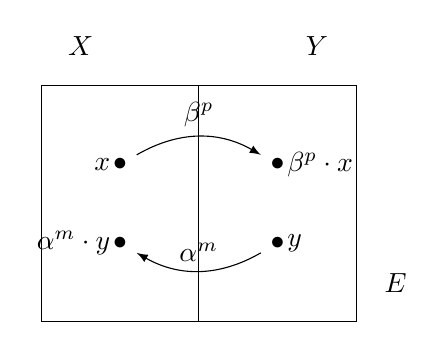
\begin{tikzpicture}
      \draw (0,0) rectangle (4, 3);
      \draw (2, 3) -- (2, 0);
      \draw (0.5, 3.5) node{$X$};
      \draw (3.5, 3.5) node{$Y$};
      \draw (4.5, 0.5) node{$E$};
      \node (x1) at (1, 2) {$\bullet$};
      \node (x2) at (3, 2) {$\bullet$};
      \node (y1) at (1, 1) {$\bullet$};
      \node (y2) at (3, 1) {$\bullet$};
      \draw (x1) node[left] {$x$};
      \draw (x2) node[right] {$\beta^p \cdot x$};
      \draw (y1) node[left] {$\alpha^m \cdot y$};
      \draw (y2) node[right] {$y$};
      \draw[->, >=latex] (x1) to [bend left] node [midway, above] {$\beta^p$} (x2);
      \draw[<-, >=latex] (y1) to [bend right] node [midway, above] {$\alpha^m$} (y2);
    \end{tikzpicture}
    \caption{Illustration du Lemme du Ping-Pong}
    \label{fig:lem-ping-pong}
  \end{figure}

  \begin{preuve}[du Lemme du Ping-Pong]
    Soit $m$ un mot réduit sur $\alpha, \beta$. $m$ est de la forme
    \begin{enumerate}
    \item $m = \alpha^{h_1} \beta^{k_1} \cdots \beta^{k_{n-1}} \alpha^{h_n}$ avec $h_i, k_i \in \Z \setminus
      \{0\}$.
        Alors supposons que $m =_G 1$. Ainsi $m \cdot Y = Y$.
          \[\alpha^{h_1} \cdots \beta^{k_{n-1}} \alpha^{h_n} \cdot Y \subseteq \alpha^{h_1} \cdots
          \beta^{k_{n-1}} \cdot X \subseteq \alpha^{h_1} \cdots \alpha^{k_{n-1}} \cdot Y \subset \cdots
          \subseteq \alpha^{h_1} \cdot Y\subset X,\]
        ainsi $m \cdot Y \subset X$, ce qui est une contradiction.

      \item $m = \beta^{k_1} \cdots \beta^{k_n}$, donc $\alpha^{-h_1}m\alpha^{h_1}$ est comme au point $1$ et
        ainsi $\alpha^{-h_1} m \alpha^{h_1} \neq_G 1$ ainsi $m \neq_G 1$.

      \item Si $m = \alpha^{h_1} \cdots \beta^{k_n}$, pour $h_0 \neq h_1$ on regarde
        $\alpha^{-h_0}(\alpha^{h_1} \cdots \beta^{k_n})\alpha^{h_0}$ qui est comme au point $1$. Donc $m
        \neq_G 1$

      \item $m = \beta^{k_1} \cdots \alpha^{h_n}$ et on fait la même preuve qu'au point 3.
    \end{enumerate}
    Ainsi $m \neq 1$ et $\langle \alpha, \beta \rangle \cong \F_2$.
  \end{preuve}

  \begin{preuve}[de \ref{prop-ss-grp-sl2}]
    Exercice.

    Début de la preuve: on regarde $E = \R^2$ et on regarde l'action de $SL_2(\Z)$ sur $\R^2$. 
      \[
      \begin{pmatrix}
        a & b \\ c & d
      \end{pmatrix}
      \cdot
      \begin{pmatrix}
        x \\ y
      \end{pmatrix} = 
      \begin{pmatrix}
        ax + by\\ cx + dy
      \end{pmatrix}
      \]

      \begin{center}
        \begin{tikzpicture}
          \draw[->, >=latex] (-3, 0) -- (4, 0);
          \draw[->, >=latex] (0, -1) -- (0, 4);
          \draw[color = OliveGreen] (-1, -1) -- (4, 4);
          \draw[color = OliveGreen] (2.5, 2.5) node[scale=0.8]{$\bullet$} node[below right]{$(x,y)$};
          \draw[dashed, color = OliveGreen] (-0.5, -1) -- (2, 4);
          \draw[color = OliveGreen] (1.5,3) node[scale=0.8]{$\bullet$} node[above left]{$(ax+by,cx+dy)$};
          \draw[->, >=latex, color = OliveGreen] (2.5, 2.5) to[bend right] (1.5, 3);
        \end{tikzpicture}
      \end{center}

      où $\cdot$ représente l'action (on prend simplement la multiplication). On ne va pas utiliser seulement
      des points, mais des droites vectorielles. On prend la droite qui passe par l'origine et $(x,y) \in
      \R^2$ et on regarde l'image de cette droite par l'action, qui est aussi une droite vectorielle. On peut
      considérer l'action sur l'ensemble des droites vectorielles dans $\R^2$ qui est l'espace projectif de
      dimension 1, $\mathbb{P}\R^1$ (une droite projective peut être vue comme ``demi-cercle'' où $A = B$).
      Il faut donc montrer que $X$ et $Y$ satisfont l'hypothèse du Lemme du Ping-Pong. 

      \begin{center}
        \begin{tikzpicture}
          \draw (-5, 0) -- (5, 0);
          \draw (3, 0) arc(0:180:3);
          \draw (-3, 0) node[below]{$A$};
          \draw (3, 0) node[below]{$B$};
          \draw (0,0) node[above]{$O$};
          \draw (-4, 4) -- (0,0) -- (4,4);
          \draw (-3, 1) node[above left]{$Y$};
          \draw (3, 1) node[above right]{$Y$};
          \draw (0, 3) node[above] {$X$};
          \draw (4,4) node[above right]{$\mathbb{P}\R^1$};
        \end{tikzpicture}
      \end{center}

  \end{preuve}

  \begin{rem}
    On trouve des groupes libres très souvent dans les groupes linéaires.
  \end{rem}

  \begin{theo}[``Alternative de Tietze'', 1971]
    Soit $G$ un groupe linéaire, c'est-à-dire un sous-groupe de $GL_n(\C)$ pour un certain $n \geq 1$. On a
    l'alternative:
    \begin{itemize}
    \item ou bien $G$ est virtuellement résoluble;
    \item ou bien $G$ contient $\F_2$ comme sous-groupe.
    \end{itemize}
  \end{theo}

  \begin{ex}
    Considérons $\mathrm{Homeo}(\R) = \{\phi: \R \to \R\, |\, \phi \text{est continue et
      bijective}\}$. $\mathrm{Homeo}(\R)$ contient beaucoup de groupes libres. 
    \begin{equation*}
      \begin{cases}
        f(x) &= x^p, \text{ $p$ premier impair,}\\
        g(x) &= x+1.
      \end{cases}
    \end{equation*}
    Alors $\langle f(x), g(x)\rangle \cong \F_2 $ (la preuve est très difficile).
  \end{ex}
  
  

  




%%% Local Variables:
%%% mode: latex
%%% TeX-master: "../GAC_cours.tex" 
%%% End: